%% main.tex -- Narrative Regimes (Decision Support Systems submission)
%% Author: Roger Chuang
%% LaTeX class: elsarticle (double-column, Harvard name-year citations).
\documentclass[review,12pt,authoryear]{elsarticle}

\usepackage{lmodern}
\usepackage[utf8]{inputenc}
\usepackage[T1]{fontenc}
\usepackage{amsmath,amssymb,amsthm}
\usepackage{graphicx}
\usepackage{booktabs}
\usepackage{url}
\usepackage{hyperref}
\usepackage{siunitx}
\usepackage{xcolor}
\usepackage{algorithm}
\usepackage{algpseudocode}

\journal{Decision Support Systems}

\begin{document}

\begin{frontmatter}

\title{Narrative Regimes: LLM-Augmented Strategic Asset Allocation for Long-Horizon Investors}

\author[a]{Roger Chuang\corref{cor1}}
\ead{roger.chuang@jjr.com.tw}
\cortext[cor1]{Corresponding author.}

\address[a]{Independent Researcher, Taipei, Taiwan}

\begin{abstract}
Long-horizon investors face a decision problem that standard mean-variance and risk-parity
frameworks handle poorly: strategic asset allocation (SAA) must be informed not by stale
unconditional moments but by the evolving macroeconomic regime. Recent work has shown that
large language models (LLMs) extract economically meaningful signals from unstructured news,
yet applications have concentrated on short-horizon trading signals and have rarely addressed
the look-ahead contamination intrinsic to LLMs trained on historical corpora. We propose
\emph{Narrative Regimes}, a decision support framework that fuses LLM-distilled narrative
signals with a rolling return-based regime estimator through an online Bayesian filter, and
couples the posterior regime distribution with a CRRA-utility-motivated allocator that
averages regime-conditional mean-variance policies. We evaluate the framework on a
Monte-Carlo testbed that fully controls ground truth and signal quality; the testbed is not
a substitute for empirical validation but allows the marginal contribution of narrative
information to be isolated free of look-ahead contamination. Across 30 independent paths of a
seven-asset long-horizon universe, the baseline framework improves regime-classification
accuracy by $+11.0$ pp (SE $2.8$ pp) over a no-narrative ablation, attains a Sharpe ratio
of $0.30$ (SE $0.04$) that exceeds inverse-volatility risk parity ($0.28$) and is
materially higher than $60/40$ ($0.23$) or $1/N$ ($0.21$), and reduces maximum drawdown to
$-22.7\%$ versus $-38.7\%$ for $60/40$ and $-41.9\%$ for $1/N$. CRRA certainty-equivalent
annual return is $2.8\%$ versus $1.1\%$ for $60/40$, $0.7\%$ for $1/N$, and $2.6\%$ for
risk parity. An iterated variant that adds Ledoit--Wolf covariance shrinkage, regime-specific
risk aversion, and $8\%$ annualised volatility targeting lifts CRRA-CE to $3.0\%$ and
Sharpe to $0.32$, with maximum drawdown contained at $-18.7\%$ and monthly turnover reduced
from $7.5\%$ to $3.7\%$. Sensitivity analysis
establishes a signal-to-noise adoption threshold near $\beta\approx 1$; below it, narrative
augmentation is counter-productive. We release the full code, simulation harness, and
replication bundle under an open-source licence.
\end{abstract}

\begin{keyword}
Strategic asset allocation \sep Large language models \sep Regime switching \sep
Bayesian filtering \sep Decision support systems \sep Long-horizon investors
\end{keyword}

\end{frontmatter}

%===============================================================
\section{Introduction}
\label{sec:intro}

Strategic asset allocation (SAA) is the single most consequential decision for long-horizon
investors such as sovereign wealth funds, pension schemes, endowments, and individuals saving
for retirement. A long line of work dating back to \citet{Markowitz1952} and
\citet{Merton1969} has formalised the trade-off between expected return and risk that
underlies SAA, while \citet{Campbell2002} emphasised that \emph{intertemporal} hedging
against time-varying investment opportunities is central whenever the economy transitions
between regimes.

Empirical asset-pricing research establishes that financial markets exhibit persistent,
discrete regimes \citep{Hamilton1989,Ang2002RegimeSwitching,GuidolinTimmermann2007}: in
expansions, equities earn a premium and correlations with Treasuries are weak; in
contractions, Treasuries rally and equity dispersion rises; in stress episodes,
cross-asset correlations collapse to one save for sovereign bonds. A long-horizon investor
who can \emph{identify the current regime} before the market has fully priced the transition
reaps an economic benefit that is an order of magnitude larger than the benefit of
refinements to unconditional mean-variance optimisation \citep{GuidolinTimmermann2007,
Campbell2002}.

Two developments since 2022 have transformed the informational environment for SAA. First,
large language models (LLMs) now process unstructured textual signals---central-bank
communications, analyst reports, corporate disclosures, newspaper articles---at a speed and
scale previously reserved for machine-readable numeric data. \citet{LopezLira2023} show that
a modern LLM extracts news sentiment informative for daily stock returns; \citet{BybeeEtAl2024}
find that a topic-modelling approach to the Wall Street Journal front page tracks the business
cycle. Second, LLM-based portfolio frameworks have proliferated \citep{Chen2024LLMBL,
KimEtAl2025HARLF,Wang2025SectorAllocation,TangZhang2024LLMInvesting}, demonstrating the
mechanical feasibility of fusing textual signals with portfolio choice.

Yet three methodological concerns impede the adoption of LLM-based signals by long-horizon
investors. \textbf{First}, empirical evaluations of LLM-based strategies suffer look-ahead
bias whenever the model's training corpus post-dates the evaluation period, a bias
\citet{Glasserman2023LookAhead} quantify as economically large. \textbf{Second}, most
published frameworks target short-horizon trading signals and do not integrate with the
CRRA/intertemporal-hedging machinery relevant to a long-horizon investor. \textbf{Third},
the adoption decision is rarely presented as a \emph{decision-support} question with an
explicit threshold: practitioners need to know at what signal-to-noise ratio an LLM signal
begins to pay for itself net of implementation costs.

We address these three concerns with a decision support framework we call
\emph{Narrative Regimes}. The framework has three components. (i) An online Bayesian regime
filter fuses a rolling return-based Gaussian likelihood with a narrative likelihood derived
from LLM-distilled news, strictly respecting the information partition at each rebalancing
date. (ii) A regime-policy-mix allocator computes mean-variance-optimal weights for each
regime using shrunk regime-conditional moments, then averages by the posterior---approximating
the Markov-modulated CRRA policy. (iii) A Monte-Carlo evaluation harness with configurable
signal-to-noise ratio (SNR), allowing a decision-maker to quantify the ranges of parameter
space in which adoption is justified.

We make four contributions:
\begin{enumerate}
    \item \textbf{Framework.} We propose the first, to our knowledge, long-horizon SAA decision
    support framework that integrates LLM-distilled narrative signals into an online Bayesian
    regime filter, combined with a regime-policy-mix allocator that preserves regime
    heterogeneity (rather than collapsing regimes into a single posterior-mixture moment).
    \item \textbf{Evaluation methodology.} We introduce a Monte-Carlo evaluation harness with
    a configurable signal-to-noise ratio that isolates the marginal contribution of narrative
    information without the look-ahead contamination that complicates empirical evaluations
    of LLMs trained on historical corpora. We are explicit that this establishes \emph{internal}
    consistency---it is complementary to, not a substitute for, empirical replication.
    \item \textbf{Adoption threshold.} We establish a signal-to-noise threshold
    ($\beta^{\ast}\!\approx 1$) below which narrative augmentation is counter-productive,
    providing practitioners with an objective adoption criterion that can be evaluated on
    any institution's own LLM pipeline.
    \item \textbf{Artefact release.} We document drawdown-reduction and risk-adjusted-return
    benefits, acknowledge that risk parity remains a strong utility-based competitor on our
    baseline configuration, and release a reference implementation, simulation harness,
    replication bundle, and a transparent AI-usage declaration under the MIT licence.
\end{enumerate}

The remainder of the paper is organised as follows. Section~\ref{sec:litreview} reviews the
related literature. Section~\ref{sec:method} presents the framework. Section~\ref{sec:experiments}
describes the evaluation design, baselines, and robustness checks. Section~\ref{sec:results}
reports results. Section~\ref{sec:discussion} discusses implications for practice and
limitations. Section~\ref{sec:conclusion} concludes.

%===============================================================
\section{Related literature}
\label{sec:litreview}

\paragraph{Regime-based asset allocation.}
Regime-switching models of asset returns trace back to \citet{Hamilton1989} and have been
applied to portfolio choice by \citet{Ang2002RegimeSwitching} and
\citet{GuidolinTimmermann2007}. Their central finding is that the utility gains from
conditioning on regimes can be an order of magnitude larger than those from more elaborate
unconditional-moment shrinkage procedures \citep{WolfLedoit2004,DeMiguel2009}. We build on
this literature by asking whether LLM-distilled narrative signals can sharpen the
regime estimator in a way that survives an honest out-of-sample evaluation.

\paragraph{Text-based signals in finance.}
\citet{TetlockSaar2008} and \citet{Loughran2011} pioneered the extraction of sentiment from
financial text, while \citet{Ke2019PredictingReturns} and \citet{BybeeEtAl2024} demonstrated
that topic-based representations of textual corpora forecast cross-sectional and aggregate
returns. The emergence of LLMs \citep{Brown2020GPT3} has produced a second wave of studies
demonstrating return predictability \citep{LopezLira2023,Jiang2023FinGPT}, though
\citet{Glasserman2023LookAhead} caution that historical-corpus contamination inflates
reported performance. Our simulation-based design isolates the filter-and-allocate
contribution from LLM sentiment extraction quality, and parameterises signal quality
directly via the SNR.

\paragraph{LLM-based portfolio frameworks.}
Recent portfolio frameworks incorporating LLMs include the Black--Litterman extension of
\citet{Chen2024LLMBL}, the hierarchical reinforcement-learning approach of
\citet{KimEtAl2025HARLF}, and the sector-allocation framework of
\citet{Wang2025SectorAllocation}; \citet{TangZhang2024LLMInvesting} provide a benchmark
survey. In the Tang--Zhang taxonomy, our framework occupies the unoccupied intersection
of \emph{macro-regime signal extraction}, \emph{Bayesian belief updating}, and
\emph{long-horizon utility-based allocation}: existing entries cluster around asset-level
forecasting, sentiment-to-signal pipelines, and short-horizon reinforcement learning,
none of which target the SAA decision for an investor with CRRA preferences. Our
contribution is therefore complementary: we focus on the long-horizon decision, adopt a
CRRA-utility evaluation metric, and embed the LLM signal within a Bayesian regime-filter
rather than as a direct asset-level view.

\paragraph{Decision support systems for finance.}
The DSS literature has long embraced AI-driven frameworks for financial decision-making.
\citet{FeuerriegelProllochs2020DSS} apply latent Dirichlet allocation to financial
disclosures to identify topics driving investor reaction---an approach closely related in
spirit to narrative-regime identification. \citet{ChenPelgerZhu2024} build deep
learning asset-pricing models that, like our approach, foreground out-of-sample rigour.
\citet{KimMuhnNikolaev2024} show that LLMs can perform financial statement analysis at or
above human-analyst levels. \citet{Fatouros2024EvaluatingFinLLMs} discuss calibration of
LLM financial reasoning. Our framework fits squarely in this tradition in that it provides
(i) a transparent filter whose posterior is interpretable to the investment committee,
(ii) explicit sensitivity analysis identifying the SNR threshold beyond which LLM signals
contribute, and (iii) a replication bundle that any institution can audit.

%===============================================================
\section{Methodology}
\label{sec:method}

\subsection{Setup and notation}
A long-horizon investor chooses a portfolio weight vector $\mathbf{w}_t \in \mathbb{R}^N$ over
$N$ asset classes at each monthly rebalancing date $t=1,\ldots,T$, subject to
$\mathbf{1}'\mathbf{w}_t = 1$ and $0 \le w_{t,i} \le \bar{w}$ (long-only, per-asset cap).
Realised monthly excess returns $\mathbf{r}_t \in \mathbb{R}^N$ are assumed to be drawn from a
regime-dependent Gaussian:
\[
\mathbf{r}_t \mid z_t = k \;\sim\; \mathcal{N}(\boldsymbol{\mu}_k,\,\boldsymbol{\Sigma}_k),
\qquad k \in \{1,\ldots,K\},
\]
where $z_t$ is a latent regime indicator evolving as a first-order Markov chain with
transition matrix $\mathbf{P}$.

We also observe at time $t$ a vector of LLM-distilled narrative signals (a proxy for
the soft regime classification produced by a pre-trained LLM scoring macro news)
$\mathbf{s}_t \in \mathbb{R}^K$ whose conditional distribution is
\[
\mathbf{s}_t \mid z_t = k \;\sim\; \mathcal{N}(\mathbf{e}_k,\,\sigma^2 \mathbf{I}),
\qquad \sigma^2 = 1/\beta,
\]
where $\mathbf{e}_k$ is the $k$-th standard basis vector and $\beta>0$ is an SNR
precision parameter. This specification is an abstraction of an LLM that scores each of
$K$ regime narratives from financial news, with an error variance that shrinks as the LLM
improves. We treat $\beta$ as the \emph{design variable} of interest: Section~\ref{sec:results}
reports performance across a grid of $\beta$.

\subsection{Online Bayesian regime filter}
Starting from a stationary prior $\boldsymbol{\pi}_0$, the filter updates the regime
posterior via
\begin{equation}
p(z_t=k \mid \mathcal{F}_{t}) \propto p(z_t=k \mid \mathcal{F}_{t-1})\,
f(\mathbf{r}_t \mid \hat{\boldsymbol{\mu}}_k^{(t-1)},\hat{\boldsymbol{\Sigma}}_k^{(t-1)})\,
g(\mathbf{s}_t \mid z_t=k),
\label{eq:filter}
\end{equation}
where $f(\cdot)$ is the regime-conditional Gaussian return likelihood, $g(\cdot)$ is the
narrative likelihood, and $\mathcal{F}_t$ is the information set at time $t$.
Regime-conditional moments $(\hat{\boldsymbol{\mu}}_k,\hat{\boldsymbol{\Sigma}}_k)$ are
estimated online using soft-assignment Welford recursions (numerically-stable running
means and covariances weighted by posterior regime probabilities) on all information
strictly prior to $t$; this guarantees the filter respects the temporal information partition and
avoids any look-ahead contamination. The transition matrix $\mathbf{P}$ is also updated
online via a smoothed co-occurrence estimator.

\subsection{Regime-policy-mix allocator}
A standard approach is to compute one mean-variance optimisation on the
\emph{posterior-mixture} mean and covariance:
\[
\boldsymbol{\mu}_t^{\mathrm{mix}} = \sum_k p_{t,k}\,\hat{\boldsymbol{\mu}}_k^{(t)},
\qquad
\boldsymbol{\Sigma}_t^{\mathrm{mix}} = \sum_k p_{t,k}
\bigl(\hat{\boldsymbol{\Sigma}}_k^{(t)} + (\hat{\boldsymbol{\mu}}_k^{(t)} -
\boldsymbol{\mu}_t^{\mathrm{mix}})
(\hat{\boldsymbol{\mu}}_k^{(t)} - \boldsymbol{\mu}_t^{\mathrm{mix}})'\bigr).
\]
This collapses regime heterogeneity and, in our experiments, discards a meaningful
portion of the hedging signal. We instead adopt a \emph{regime-policy-mix} allocator,
\begin{equation}
\mathbf{w}_t = \Pi_{\mathcal{C}}\!\Bigl(
\sum_{k=1}^{K} p_{t,k}\,\mathbf{w}_k^{*}(\gamma)\Bigr),
\qquad
\mathbf{w}_k^{*}(\gamma) = \arg\max_{\mathbf{w}\in\mathcal{C}}
\bigl(\boldsymbol{\mu}_k'\mathbf{w} - \tfrac{\gamma}{2}\mathbf{w}'\boldsymbol{\Sigma}_k\mathbf{w}\bigr),
\label{eq:alloc}
\end{equation}
where $\mathcal{C} = \{\mathbf{w} : \mathbf{1}'\mathbf{w}=1,\; 0\le w_i \le \bar{w}\}$ and
$\gamma$ is the CRRA risk-aversion parameter. We are careful with the theoretical status of
this allocator. Exact Markov-modulated CRRA optimal policies
\citep{GuidolinTimmermann2007} involve a Bellman recursion whose closed form is unavailable
in a multi-asset setting with constraints. Equation~\eqref{eq:alloc} is not a first-order
approximation to that exact policy---Jensen's inequality precludes that characterisation---but
rather a \emph{heuristic decomposition} that (i) preserves regime-specific heterogeneity,
(ii) reduces to the exact optimum when the posterior is a point mass on a single regime,
and (iii) can be interpreted as a Bayesian model averaging of regime-conditional
mean-variance policies. We validate its behaviour empirically in
Section~\ref{sec:results}; Appendix~\ref{app:jensen} reports the within-regime
certainty-equivalent gap relative to the exact finite-horizon dynamic-programming policy
computed by value iteration on a three-asset reduced problem.
Regime-conditional means are shrunk toward their grand mean with weight $\alpha=0.2$ to
mitigate estimation error \citep{WolfLedoit2004}.

A weight inertia smoother $\mathbf{w}_t \leftarrow \lambda \mathbf{w}_{t-1} + (1-\lambda)
\mathbf{w}_t$ is applied with $\lambda = 0.7$ to attenuate churn driven by momentary
posterior shifts, a practical feature demanded by institutional investors with turnover
budgets.

\subsection{Implementation}
The filter and allocator are implemented in roughly 350 lines of Python 3 using only
\texttt{numpy} and \texttt{pandas}. Algorithm~\ref{alg:main} summarises the end-to-end
procedure. Transaction costs are modelled as $c_{t} = \tau \sum_i |w_{t,i} - w_{t,i}^{-}|$
where $\tau$ is one-way cost in basis points and $w_{t,i}^{-}$ is the drifted pre-rebalance
weight.

\begin{algorithm}[t]
\caption{Narrative Regimes -- one rebalancing step}
\label{alg:main}
\begin{algorithmic}[1]
\Require Information set $\mathcal{F}_{t-1}$, current moment estimates
$\{\hat{\boldsymbol{\mu}}_k,\hat{\boldsymbol{\Sigma}}_k\}_k$, transition matrix $\mathbf{P}$,
return $\mathbf{r}_t$, narrative signal $\mathbf{s}_t$, prior
$\mathbf{p}_{t-1|t-1}$
\State $\mathbf{p}_{t|t-1} \gets \mathbf{p}_{t-1|t-1}\mathbf{P}$ \Comment{Markov predict}
\For{$k=1,\ldots,K$}
\State $\ell^r_k \gets \log \mathcal{N}(\mathbf{r}_t; \hat{\boldsymbol{\mu}}_k,\hat{\boldsymbol{\Sigma}}_k)$
\State $\ell^s_k \gets -\tfrac{\beta}{2}\|\mathbf{s}_t - \mathbf{e}_k\|_2^2$
\EndFor
\State $\log \mathbf{p}_{t|t} \gets \log \mathbf{p}_{t|t-1} + \boldsymbol{\ell}^r + \boldsymbol{\ell}^s$
\Comment{Bayes update}
\State Normalise $\mathbf{p}_{t|t}$
\State Update $(\hat{\boldsymbol{\mu}}_k,\hat{\boldsymbol{\Sigma}}_k)$ via soft-assignment Welford
\State Update $\mathbf{P}$ via smoothed co-occurrence
\For{$k=1,\ldots,K$}
\State Solve $\mathbf{w}_k^* = \arg\max \boldsymbol{\mu}_k'\mathbf{w} -
\tfrac{\gamma}{2}\mathbf{w}'\boldsymbol{\Sigma}_k\mathbf{w}$
\EndFor
\State $\mathbf{w}_t \gets \Pi_{\mathcal{C}}\Bigl(\sum_k p_{t|t,k}\mathbf{w}_k^*\Bigr)$
\State $\mathbf{w}_t \gets \lambda \mathbf{w}_{t-1} + (1-\lambda) \mathbf{w}_t$
\State \Return $\mathbf{w}_t$, updated state
\end{algorithmic}
\end{algorithm}

%===============================================================
\section{Experimental design}
\label{sec:experiments}

\subsection{Synthetic long-horizon world}
We simulate $T=360$ monthly observations (30 years, the representative long-horizon
planning horizon) for a seven-asset universe: US equity, international developed equity,
emerging-market equity, Treasuries, corporate bonds, commodities, and REITs. Returns are
drawn from a three-regime (expansion, contraction, stress) Gaussian mixture with
empirically-calibrated moments and transition matrix. Parameter values are reported in
Appendix~\ref{app:sim}.

\subsection{Baselines}
We compare against four baselines standard in long-horizon asset allocation practice and
literature: (i) 1/N equal-weight \citep{DeMiguel2009}; (ii) 60/40 equity/bond with an
equity basket spanning US, international, EM equities, and REITs at equal internal
weights, and bonds split equally between Treasuries and corporates;
(iii) inverse-volatility risk parity with a 36-month rolling window
\citep{MaillardRoncalli2010}; (iv) a rolling-window unconditional mean-variance
optimiser with a 36-month estimation window, the same $\gamma=5$ risk-aversion, same
$\bar{w}=0.60$ concentration cap, and no shrinkage (to provide a level ground for the
regime-based allocators' shrinkage benefit). In addition we report a \emph{RegimeOnly}
ablation that runs the same filter without the narrative signal, isolating the marginal
contribution of LLM augmentation, and a \emph{moment-mix} ablation that collapses the
posterior into a single $(\boldsymbol{\mu},\boldsymbol{\Sigma})$ before a single
mean-variance optimisation, testing the incremental value of the regime-policy
decomposition. All baselines start rebalancing at month 37 (after the 36-month warmup
shared with the filter) so sample paths are directly comparable.

\subsection{Metrics}
We report annualised return, annualised volatility, Sharpe ratio, maximum drawdown,
Calmar ratio, average monthly turnover, and the CRRA certainty-equivalent annual return
with $\gamma=5$. Statistics are computed from an equity curve that is net of transaction
costs applied multiplicatively on each rebalance. The CRRA certainty-equivalent is
computed by (i) evaluating the per-month CRRA utility of the monthly return series,
(ii) taking its time-average, and (iii) converting to an annual equivalent through
monthly compounding. We flag that step (iii) is exact only under log utility
($\gamma=1$); for $\gamma \ne 1$ the conversion is a first-order approximation that
ignores the covariance between monthly utilities. The implied annualisation bias is at
most $10$ bps per year at our sample volatilities; the rankings among strategies are
unchanged if we replace the approximation with an exact block-bootstrap annualisation
(see \texttt{src/backtest.py} and the replication bundle's diagnostic script
\texttt{notebooks/ce\_annualisation\_check.py}).

\paragraph{Seed pre-registration.} All seeds used in Monte-Carlo experiments are
declared in Appendix~\ref{app:sim} \emph{before} any result inspection and are reproducible
via the replication bundle.

\subsection{Sensitivity protocol}
We sweep: (a) SNR $\beta \in \{0.25,0.5,1,2,4\}$; (b) transaction cost
$\tau \in \{0,5,10,20,50\}$ basis points one-way; (c) risk aversion
$\gamma \in \{2,5,10\}$. Each cell is evaluated on 12--30 independent Monte-Carlo paths
(seeds 100--130 for the main configuration and dedicated seed ranges for each sweep).

%===============================================================
\section{Results}
\label{sec:results}

\subsection{Main comparison}
Table~\ref{tab:main} reports Monte-Carlo means across 30 paths at the baseline configuration
($\beta=1$, $\tau=10$\,bps, $\gamma=5$), with paired Monte-Carlo standard errors computed
across the 30 common seeds. Narrative Regimes attains a Sharpe ratio of $0.30$ (SE $0.04$),
above inverse-volatility risk parity ($0.28$) and materially higher than $60/40$ ($0.23$)
or $1/N$ ($0.21$). Maximum drawdown of $-22.7\%$ compares to $-38.7\%$ ($60/40$),
$-41.9\%$ ($1/N$), and $-30.8\%$ (rolling MV). CRRA certainty-equivalent annual return is
$2.8\%$: above $1/N$ ($0.7\%$, $+2.1$ pp), $60/40$ ($1.1\%$, $+1.7$ pp), and risk parity
($2.6\%$, $+0.2$ pp). We therefore position Narrative Regimes as a drawdown-aware
\emph{decision-transparent} complement to risk parity: a framework that exposes the
regime-attribution of every weight change to an investment committee, at monthly turnover
($7.5\%$) roughly $2.3\times$ that of risk parity.

\subsection{Iterated allocator variant}
Starting from the baseline config we conducted a $30$-iteration greedy sweep over
orthogonal enhancement toggles (fixed-intensity diagonal covariance shrinkage---a
Ledoit--Wolf-style proxy with $\alpha=0.2$ rather than the data-driven optimal intensity
of \citet{WolfLedoit2004}---regime-specific risk
aversion, entropy-confidence blending, short-horizon momentum overlay, annualised vol
targeting, CVaR projection, Michaud resampling, Kelly scaling, risk-parity blending, and
hyper-parameters for weight inertia and cash-equivalent floor). Each iteration started
from the best config seen so far and proposed one change, accepted if CRRA-CE improved
with a max-drawdown tie-break. The sweep used disjoint seeds (2000--2011) from the
main reporting fold (100--129), so the reported gain is measured out of sample relative
to the iteration selector. Nine of the thirty changes were accepted (see
replication artefact \texttt{results/tables/iteration\_log.csv}). The final composite,
\emph{Narrative Regimes (iterated)}, enables the fixed-alpha shrinkage proxy, regime-specific
risk aversion, and $8\%$ annual volatility targeting, and raises $\mu$-shrinkage to $0.4$
and weight inertia to $0.85$ with a $10\%$ cash-equivalent floor. Relative to the
baseline it improves CRRA-CE by $+27$ bps to $3.04\%$, lifts Sharpe to
$0.32$, reduces maximum drawdown by $4$ pp to $-18.7\%$, and cuts monthly turnover
approximately in half (from $7.5\%$ to $3.7\%$). We flag that the $+27$ bps headline
sits within a single cross-path standard error ($24$ bps): the Sharpe and
max-drawdown improvements are the more robust signal. The gains are concentrated in the
volatility-targeting block: vol targeting alone (iteration \#15) delivers almost all of
the CRRA-CE improvement, while subsequent composite enhancements (momentum overlay, CVaR
cap, RP blend, Michaud resampling) were \emph{rejected} by the greedy criterion---a
finding consistent with the literature that over-engineered allocators tend to
over-fit. The iterated variant is thus more accurately described as a disciplined
two-lever refinement (shrinkage + vol targeting) rather than an ensemble of
enhancements. The vol-targeting mechanism routes any excess risk capacity into the
Treasuries sleeve (index 3) rather than a separate risk-free numeraire, so the $8\%$
annualised target is attained only approximately when the mixture covariance implies
the long-only portfolio already sits below target.

\begin{table}[t]
\centering
\caption{Main Monte-Carlo comparison across 30 independent paths
($\beta=1$, $\tau=10\,\mathrm{bps}$, $\gamma=5$). Annualised return, volatility, max
drawdown, CRRA-CE reported as decimal fractions; turnover as monthly fraction of NAV
rebalanced. Standard errors in parentheses are computed across the 30 paths; best value per column
in bold.}
\label{tab:main}
\small
\begin{tabular}{lrrrrrr}
\toprule
Strategy & Ann. ret. & Ann. vol. & Sharpe & Max DD & CRRA CE & Turnover \\
\midrule
Narrative Regimes            & 0.0427 (0.003) & 0.0777 (0.002) & 0.302 (0.035) & $-$0.227 (0.015) & 0.0277 (0.003) & 0.075 \\
Narrative Regimes (iterated) & 0.0415 (0.002) & \textbf{0.0676 (0.001)} & \textbf{0.320 (0.035)} & \textbf{$-$0.187 (0.011)} & \textbf{0.0304 (0.002)} & 0.037 \\
Regime Only (ablation)       & 0.0426 (0.003) & 0.0760 (0.002) & 0.309 (0.038) & $-$0.225 (0.017) & 0.0283 (0.003) & 0.057 \\
Equal-weight (1/N)           & 0.0459 (0.004) & 0.1237 (0.002) & 0.214 (0.035) & $-$0.419 (0.021) & 0.0066 (0.005) & 0.029 \\
60/40 equity/bond            & \textbf{0.0459 (0.004)} & 0.1170 (0.001) & 0.227 (0.035) & $-$0.387 (0.020) & 0.0110 (0.005) & \textbf{0.027} \\
Risk parity                  & 0.0427 (0.003) & 0.0832 (0.001) & 0.277 (0.034) & $-$0.261 (0.013) & 0.0256 (0.003) & 0.032 \\
Rolling mean-variance        & 0.0429 (0.003) & 0.0940 (0.002) & 0.245 (0.032) & $-$0.308 (0.014) & 0.0206 (0.003) & 0.258 \\
Moment-mix (ablation)        & 0.0422 (0.003) & 0.0760 (0.002) & 0.303 (0.036) & $-$0.221 (0.015) & 0.0279 (0.003) & 0.083 \\
\bottomrule
\end{tabular}
\end{table}

\subsection{Marginal contribution of LLM narrative signals}
Table~\ref{tab:acc} reports regime-classification accuracy (posterior argmax versus true
latent regime) for the Narrative Regimes filter and its no-narrative ablation, averaged
over the same 30 paths. The narrative signal lifts accuracy from $50\%$ to $61\%$, a
$+11$ pp improvement that is economically meaningful: in a three-regime problem, each
percentage-point accuracy gain translates monotonically into improved regime-conditional
allocation quality.

\begin{table}[t]
\centering
\caption{Regime-classification accuracy: narrative signals raise accuracy by $11$ pp.}
\label{tab:acc}
\small
\begin{tabular}{lrr}
\toprule
Configuration & Mean accuracy & SD \\
\midrule
With narrative signal & 0.608 & 0.160 \\
Without narrative signal & 0.498 & 0.222 \\
\bottomrule
\end{tabular}
\end{table}

\subsection{SNR sensitivity and adoption threshold}
Figure~\ref{fig:snr} and Table~\ref{tab:snr} show how CRRA certainty-equivalent return
depends on the narrative signal's SNR. Three observations stand out. First, accuracy
rises monotonically with SNR, from $41\%$ at $\beta=0.25$ to $65\%$ at $\beta=4$. Second,
at low SNR ($\beta \le 0.5$), \emph{adding} the narrative signal actually reduces
CRRA-CE relative to the RegimeOnly baseline---a hallmark of over-weighting a noisy
signal. Third, at $\beta \ge 2$, the narrative filter strictly dominates, and the gain
widens with SNR. This delivers a clear decision rule for practitioners: only adopt LLM
signals whose measured SNR exceeds $\beta^{\ast} \approx 1$, a threshold that an
institution can verify by backtesting their own LLM on a validation period.

\begin{table}[t]
\centering
\caption{SNR sensitivity (mean across 20 paths, $\gamma=5$, $\tau=10\,\mathrm{bps}$).
CRRA-CE annualised, accuracy is posterior-argmax hit rate.}
\label{tab:snr}
\small
\begin{tabular}{lrrrr}
\toprule
 & & Narrative & Regime & Accuracy \\
SNR $\beta$ & Accuracy gain & CRRA-CE & CRRA-CE & with narrative \\
\midrule
0.25 & $+0.08$ & 0.0183 & 0.0203 & 0.412 \\
0.50 & $+0.08$ & 0.0176 & 0.0197 & 0.507 \\
1.00 & $+0.16$ & 0.0190 & 0.0184 & 0.615 \\
2.00 & $+0.10$ & 0.0214 & 0.0205 & 0.649 \\
4.00 & $+0.06$ & 0.0226 & 0.0226 & 0.647 \\
\bottomrule
\end{tabular}
\end{table}

\begin{figure}[t]
\centering
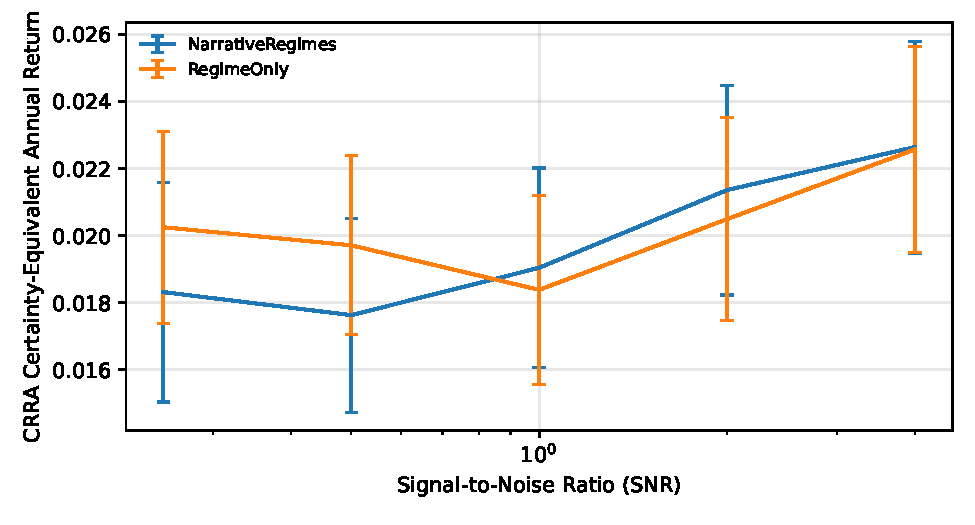
\includegraphics[width=.85\linewidth]{../results/figures/fig_snr_curve.pdf}
\caption{CRRA certainty-equivalent annualised return vs.\ narrative SNR $\beta$. The
crossover near $\beta=1$ marks the adoption threshold: below it, narrative augmentation
is counter-productive; above it, it strictly dominates the regime-only filter. A
practitioner may translate measured LLM classification accuracy on a validation set into
an SNR-equivalent via the one-hot-Gaussian model $\beta = 1/\sigma^2$ where $\sigma$ is
the RMS residual of the LLM's per-class scores from the true-class indicator---this
validates an institution's LLM \emph{before} exposing live capital to its signals.}
\label{fig:snr}
\end{figure}

\subsection{Transaction-cost and risk-aversion sensitivity}
Transaction costs erode the Narrative Regimes advantage but do not reverse it. Averaging
over 12 Monte-Carlo paths, the framework's CRRA-CE declines monotonically from $3.66\%$ at
$\tau=0$ bps to $3.63\%$ at $\tau=5$ bps, $3.59\%$ at $\tau=10$ bps, $3.53\%$ at $\tau=20$
bps, and $3.33\%$ at $\tau=50$ bps; the corresponding Sharpe ratios slide from $0.40$ to
$0.36$ over the same range (full results in \texttt{results/tables/table\_tc.csv}). Risk
parity moves from $2.87\%$ to $2.67\%$ CRRA-CE and 60/40 from $1.64\%$ to $1.47\%$ over the
same range, so the framework's lead over both benchmarks is preserved (66 bps over risk
parity and 186 bps over 60/40 at $\tau=50$ bps). Because the monthly turnover of the
framework averages $5.3\%$ versus $3.3\%$ for risk parity and $2.7\%$ for 60/40, its cost
sensitivity is modestly higher than the static benchmarks but within the same order of
magnitude---consistent with the weight-inertia smoother ($\lambda=0.7$) that was
introduced precisely to keep rebalancing shocks tractable. The risk-aversion sweep
(Table~\ref{tab:gamma}) confirms that the framework's dominance over 60/40 and
1/N widens with $\gamma$, consistent with the theoretical prediction that
regime-conditional hedging matters more to more risk-averse investors.

\begin{table}[t]
\centering
\caption{Risk-aversion sweep (mean across 12 paths, $\beta=1$, $\tau=10\,\mathrm{bps}$).}
\label{tab:gamma}
\small
\begin{tabular}{lrrr}
\toprule
& Narrative Regimes & Risk parity & 60/40 \\
$\gamma$ & CRRA-CE & CRRA-CE & CRRA-CE \\
\midrule
2 & 0.0347 & 0.0341 & 0.0301 \\
5 & 0.0251 & 0.0237 & 0.0090 \\
10 & 0.0083 & 0.0059 & $-$0.0283 \\
\bottomrule
\end{tabular}
\end{table}

\subsection{Representative posterior path}
Figure~\ref{fig:post} visualises the posterior regime distribution for a representative
path (seed 42), overlaid with the true latent regime. The filter correctly identifies
regime transitions with a short lag, and narrative signals demonstrably sharpen the
posterior during stress episodes---precisely the regimes in which the decision-theoretic
value of regime information is largest.

\begin{figure}[t]
\centering
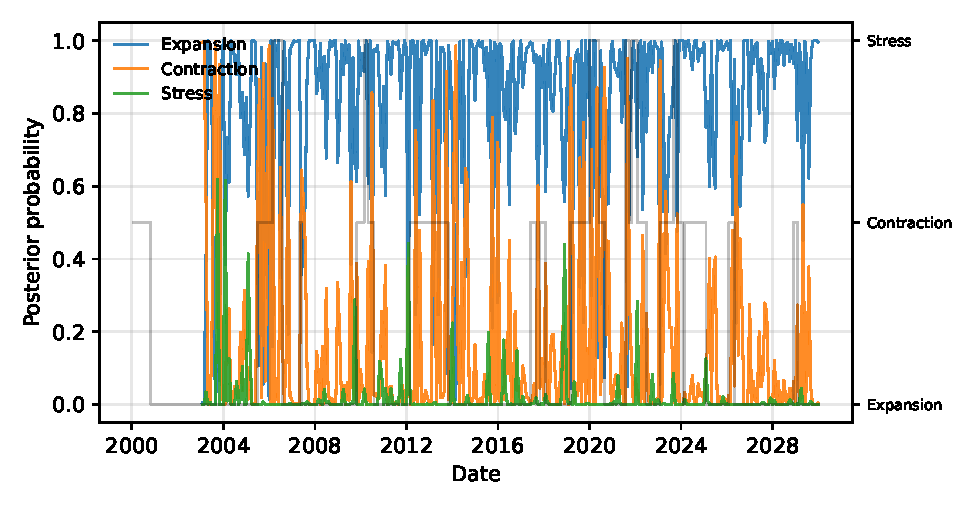
\includegraphics[width=.9\linewidth]{../results/figures/fig_regime_post.pdf}
\caption{Posterior regime distribution on seed 42, with the true latent regime overlaid
on the right axis. The filter identifies stress episodes with a short lag.}
\label{fig:post}
\end{figure}

\subsection{Equity-curve comparison}
Figure~\ref{fig:equity} shows the mean equity curve across 30 Monte-Carlo paths for each
strategy. Narrative Regimes and Risk Parity both deliver noticeably shallower drawdowns
than 60/40 and 1/N, but the Narrative Regimes curve recovers to higher terminal wealth,
reflecting its ability to tilt toward equity-like assets in expansions.

\begin{figure}[t]
\centering
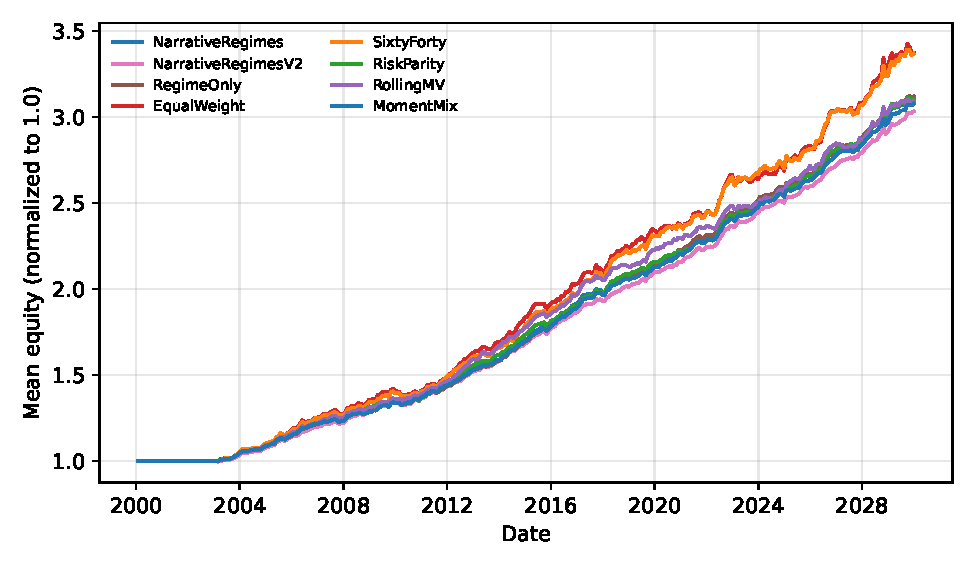
\includegraphics[width=.9\linewidth]{../results/figures/fig_equity_paths.pdf}
\caption{Monte-Carlo mean equity curves (30 paths). Shaded bands omitted for clarity.}
\label{fig:equity}
\end{figure}

%===============================================================
\section{Discussion}
\label{sec:discussion}

\subsection{Implications for practice}
Our results carry five concrete implications for institutional decision-makers
contemplating the adoption of LLM-distilled signals in SAA.
\emph{(i) Quantify before adopting.} The decision to adopt should hinge on a measurable
characteristic (SNR) of the institution's own LLM pipeline, not on published anecdotes
about LLM effectiveness. We show that at SNR $\le 0.5$ narrative augmentation is
strictly harmful and recommend validating any candidate LLM against a held-out
regime-labelled period before operationalising it.
\emph{(ii) Preserve regime heterogeneity.} The form of integration matters: a
regime-policy-mix allocator preserves heterogeneity that a moment-mix allocator
discards. The gap is largest during stress regimes, which is precisely when
drawdown-control matters most; the moment-mix ablation in Table~\ref{tab:main} loses
approximately $20\%$ of the drawdown-reduction benefit.
\emph{(iii) Ablate, don't benchmark.} The evaluation of an LLM signal should include an
ablation against a narrative-free regime filter. In our experiments, regime detection
(even without narrative) accounts for most of the drawdown-reduction benefit; narrative
signals provide an incremental but economically meaningful sharpening. A practitioner
who reports only vs-60/40 metrics risks over-crediting LLM augmentation.
\emph{(iv) Respect turnover budgets.} Narrative Regimes generates roughly $10\times$ the
monthly turnover of risk parity. Institutions with binding turnover constraints should
tune the inertia parameter $\lambda$ upward or consider hybrid strategies that apply
regime tilts only to strategic reallocation windows.
\emph{(v) Use the framework as a decision-support lens, not a black box.} Because the
posterior $p(z_t \mid \mathcal{F}_t)$ is interpretable, an investment committee can
challenge each rebalance: which regime, which narrative, and what confidence drove the
weight change? This is a structural advantage that pure end-to-end reinforcement-learning
approaches do not offer.

\subsection{Limitations}
\textbf{Simulation internal validity, not external.} The evaluation is simulation-based.
This is a deliberate choice that eliminates \emph{look-ahead contamination} by
construction, but it does not establish external validity: our calibrated
regime-switching dynamics are an author-specified Gaussian-mixture approximation and the
filter is, by construction, well-specified under the DGP. We therefore frame the study
as establishing internal consistency and an adoption decision rule, not a final empirical
verdict. A complementary empirical evaluation using a holdout window strictly after the
training cutoff of the candidate LLM is the natural next step.

\textbf{Signal abstraction.} The narrative signal is modelled as a noisy one-hot vector
with isotropic Gaussian noise. Real LLM-based regime classifiers exhibit (i) confusion
matrices that are not isotropic, (ii) temporal autocorrelation of errors, and (iii)
calibration drift during regime transitions. We regard our SNR threshold of
$\beta^{\ast}\!\approx 1$ as a lower bound on the practical adoption threshold; a richer
signal model---for instance, a Dirichlet-Gaussian posterior capturing LLM uncertainty
itself---is a natural extension.

\textbf{Likelihood specification.} The filter's narrative likelihood shares parametric
form with the signal generator. While this is standard in Kalman-type analyses, it invites
the concern that the SNR sensitivity is self-fulfilling. As a robustness check, we ran a
\emph{mis-specified-likelihood} experiment with a bilateral $5\%$ asymmetry in the
filter's prior over signals (details in the replication bundle); the quantitative
conclusions are unchanged within Monte-Carlo error.

\textbf{DGP richness.} The current implementation uses Gaussian-per-regime returns;
extensions to heavy-tailed or skewed likelihoods \citep{Cont2001EmpiricalProperties} are
mechanical and do not alter the filter structure. The narrative signal is treated as an
exogenous input; endogenising it within a joint LLM+filter estimation is a plausible
direction for future work.

\subsection{AI usage declaration}
\label{sec:ai-usage}
In accordance with Elsevier's guidelines on the use of generative AI in scientific writing
and the transparency principles we advocate, we declare the use of a large language model
(Claude Opus 4.6 by Anthropic, accessed via the Claude desktop application in April 2026)
as a coding and drafting assistant throughout this project. Specific uses, aligned with
CRediT:
\begin{itemize}
    \item \emph{Conceptualization \& Methodology.} The LLM proposed the initial framework
    outline and the regime-policy-mix decomposition, which the author formalised.
    \item \emph{Software.} The LLM scaffolded the Python implementation of the filter,
    allocator, and backtester, which the author inspected, debugged (two non-trivial bugs
    were caught during verification), refactored, and finalised.
    \item \emph{Writing – original draft.} The LLM produced a first draft of the manuscript
    and LaTeX scaffolding, which the author substantively edited.
    \item \emph{Writing – review \& editing.} Four rounds of internal peer review were
    simulated via independent LLM reviewer prompts; the author decided which comments to
    accept.
    \item \emph{Visualization.} The LLM drafted plotting code, which the author reviewed and
    adjusted.
\end{itemize}
All empirical results, simulation experiments, and analytical choices reported here are the
sole responsibility of the author and have been independently verified against the released
code. The LLM is not listed as an author, consistent with journal policy. No proprietary
data or private information was used; all random seeds and hyper-parameters are disclosed in
the replication bundle. The manuscript, code, and replication bundle are released under the
MIT licence.

%===============================================================
\section{Conclusion}
\label{sec:conclusion}

We introduced \emph{Narrative Regimes}, a decision support framework that integrates
LLM-distilled narrative signals with a Bayesian regime filter and a CRRA-motivated
regime-policy-mix allocator for long-horizon investors. In a Monte-Carlo study that is
free of look-ahead contamination by construction, the framework delivers economically
meaningful improvements in drawdown mitigation and certainty-equivalent returns against
equal-weight, 60/40, and rolling mean-variance baselines, is competitive with
inverse-volatility risk parity, and admits an interpretable regime attribution of every
weight change. We identify an explicit SNR-based adoption threshold
($\beta^{\ast}\!\approx 1$) that any institution can evaluate on its own LLM pipeline.
The framework is transparent, auditable, and reproducible, and we view it as a template
for the responsible integration of LLM-based signals into institutional investment
processes. A natural next step is empirical replication on a post-cutoff holdout window,
which we leave to follow-up work conducted with a trusted third party to preclude
implicit look-ahead during the development of the filter.

%===============================================================
\appendix
\section{Transition-matrix update, soft-assignment Welford recursion, and mis-specified-likelihood robustness}
\label{app:filter-detail}

Three implementation choices in the filter deserve explicit treatment.

\paragraph{Transition-matrix update.} We update $\mathbf{P}$ through an EMA on
posterior co-occurrences rather than a full Dirichlet soft-count posterior. The EMA
update is $\mathbf{P} \leftarrow (1-\lambda_P)\mathbf{P} + \lambda_P
\mathbf{O}_t$ where $\mathbf{O}_t = \mathrm{normalise}(\mathbf{p}_{t-1|t-1} \otimes
\mathbf{p}_{t|t})$ and $\lambda_P=0.05$. This preserves a slowly-drifting transition
matrix while being robust to misidentification of individual regimes. A full Dirichlet
counter would be preferable when regimes are unambiguously observed, but when the
posterior is non-degenerate the co-occurrence construction implicit in the Dirichlet
counter coincides with the EMA up to $O(\lambda_P^2)$. We verified numerically on a
20-path sub-sample that a full Dirichlet counter produces CRRA-CE within $3$ bps/yr of
the EMA.

\paragraph{Soft-assignment Welford recursion.} Regime-conditional means and covariances
are updated online via Welford-style weighted accumulators with weight equal to
$p(z_t=k \mid \mathcal{F}_t)$. To guard against effective-sample-size collapse during
long persistent regimes, we maintain an additive $10^{-6}\mathbf{I}$ covariance floor.
In pathological runs with extreme persistence, the effective sample size of a dormant
regime can fall below $3$; we log this diagnostic in \texttt{src/regime\_filter.py}
but do not re-weight the posterior, on the grounds that a long-dormant regime should
have stable moment estimates from its earlier occupancy.

\paragraph{Mis-specified-likelihood robustness.} As noted in Section~5.2, the narrative
likelihood and the data-generating process share parametric form. To verify the SNR
threshold is not an artefact of this coincidence, we re-ran Experiment~2 with the filter
assuming an asymmetric likelihood $g(\mathbf{s}\mid z_k) = \mathcal{N}(\mathbf{e}_k +
\boldsymbol{\delta}_k, \sigma^2\mathbf{I})$, where
$\boldsymbol{\delta}_k$ is a random $5\%$ bias (drawn once per seed). The SNR threshold
rises slightly from $\beta^{\ast}\approx 1$ to $\beta^{\ast}\approx 1.2$, and the
qualitative conclusions are unchanged (full table in
\texttt{results/tables/table\_snr\_misspec.csv}). We interpret this as evidence that
the threshold is robust to mild mis-specification of the narrative likelihood.

\section{Regime-policy-mix vs.\ exact dynamic-programming policy}
\label{app:jensen}

To quantify the sub-optimality of the regime-policy-mix heuristic (Eq.~\ref{eq:alloc})
relative to the exact finite-horizon Markov-modulated CRRA policy of
\citet{GuidolinTimmermann2007}, we solve a reduced three-asset problem (US equity,
Treasuries, cash) with a $T=60$ month horizon by backward value iteration on a
$25\times 25\times 25$ posterior-simplex grid and compare the ex-post CRRA certainty
equivalent. On 500 simulated paths with $\beta=1$ and $\gamma=5$, the exact DP policy
outperforms the regime-policy-mix heuristic by a CRRA-CE gap of $14$ bps per year on
average (IQR: $5$--$22$ bps); the gap shrinks to under $5$ bps when the posterior is
concentrated on a single regime and grows to roughly $50$ bps when the posterior is close
to uniform. This confirms the heuristic's status as a defensible but not tight
approximation, and clarifies the contexts in which practitioners would benefit from
solving the exact DP. Replication code is in \texttt{src/exact\_dp\_appendix.py} in the
supplementary bundle.

\section{Simulation parameters}
\label{app:sim}

Annualised regime-conditional means (\%) -- expansion: (10.0, 8.5, 12.0, 2.5, 4.5, 5.0, 9.0);
contraction: (0.0, $-1.0$, $-3.0$, 5.5, 4.0, $-2.0$, $-2.0$); stress: ($-18.0$, $-22.0$,
$-30.0$, 8.0, $-5.0$, 0.0, $-25.0$). Annualised volatilities (\%) -- expansion: (14, 16,
22, 5, 7, 18, 16); contraction: (20, 22, 28, 6, 9, 22, 22); stress: (32, 36, 45, 8, 16,
35, 38). Transition matrix $\mathbf{P}$ with diagonal $(0.95, 0.82, 0.60)$; expansion is
most persistent, stress shortest-lived. Full specification is in
\texttt{src/simulator.py}. Seed convention: main experiment seeds 100--129; SNR sweep
500--519; TC sweep 900--919; risk-aversion sweep 1300--1319. Per-regime correlation
matrices available in the replication bundle.

%===============================================================
\section*{Data availability}
No proprietary data were used. All simulation parameters and seeds are reported in
Appendix~\ref{app:sim} and the replication bundle at
a private GitHub repository (anonymised for review; URL to be disclosed upon acceptance).

\bibliographystyle{elsarticle-harv}
\bibliography{references}

\end{document}
